\documentclass[11pt, oneside]{article} 
\usepackage{geometry}
\geometry{letterpaper} 
\usepackage{graphicx}
	
\usepackage{amssymb}
\usepackage{amsmath}
\usepackage{parskip}
\usepackage{color}
\usepackage{hyperref}

\graphicspath{{/Users/telliott/Dropbox/Github-Math/geoproof/figures/}{/Users/telliott/Dropbox/Github-Math/figures/}}
% \begin{center} \includegraphics [scale=0.4] {gauss3.png} \end{center}


\title{Triangles relations}
\date{}

\begin{document}
\maketitle
\Large

%[my-super-duper-separator]

There are a number of interesting examples of triangles drawn inside triangles using points placed by medians or altitudes and so on.  We look at three.

\subsection*{centroid}
The first is the median.  Midpoints are marked for $\triangle ABC$ and one median is drawn (dotted line).

The midpoint criterion means that, for example, $AD = DB$ and $AE = EC$.  Since $\angle A$ is shared, $\triangle ADE \sim \triangle ABC$, with a ratio of sides of $1:2$.
\begin{center} 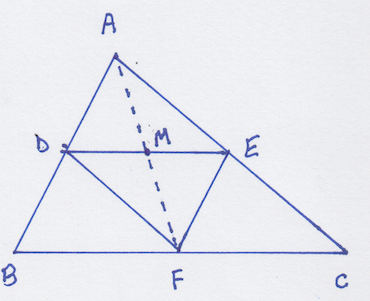
\includegraphics [scale=0.5] {T2.png} \end{center}
Symmetry or similar logic will show that $\triangle BDF$ and $\triangle EFC$ have exactly the same relationship with $\triangle ABC$.  Since the side ratios to the large triangle are all equal, we conclude that the three small triangles are not just similar but congruent.

Another way to do this is to use the midpoint relationships to show that $DE \parallel BC$.  Alternate interior angles and triangle sum of angles will give the result.

Note that $DEFB$ is a parallelogram.  It has two pairs of opposite sides equal and the shared diagonal $DF$ means we have SSS so opposing angles are equal and we have a parallelogram.  Therefore $\triangle DEF$ is congruent to the other three.

But $MF$ is a median of $\triangle DEF$.  We can draw another small triangle inside $\triangle DEF$ and it will have the same medians as $\triangle ABC$ and $\triangle DEF$.

Therefore, the centroid exists, and we could make an algebraic argument for why it lies one-third of the way from $F$ up along the median, below $M$, but we rely on our previous demonstration instead.
\begin{center} 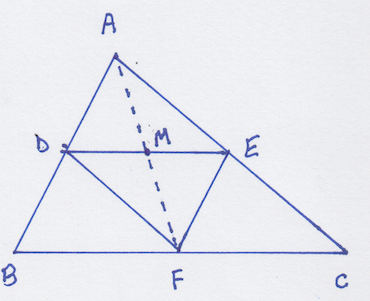
\includegraphics [scale=0.5] {T2.png} \end{center}

\subsection*{circumcenter and orthocenter}
In a triangle we draw the perpendicular bisectors of the sides.  
\begin{center} 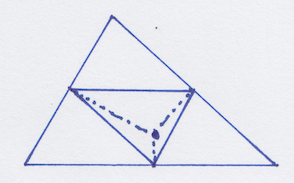
\includegraphics [scale=0.6] {T4.png} \end{center}
They meet at the circumcenter, which we know must exist, since having drawn two bisectors and finding where they meet, we know the circumcenter.

But this is the same arrangement we had in the previous diagram, we are just drawing the dotted lines in a different direction.   Hence we have the same three parallelograms and the same congruent triangles.

Since the horizontal in the middle is parallel to the base, the perpendicular bisector of the base meets that horizontal in a right angle.  It \emph{is} the altitude of the small inset triangle.  Since the circumcenter certainly exists, this is a proof that the orthocenter also exists.

\subsection*{altitudes and angle bisectors}
In the first two examples the proofs related to concurrence.  When we said that a point, whether the centroid or the orthocenter \emph{exists}, we mean that the three medians or altitudes are concurrent at that point.

In the previous example we showed that the triangle drawn to the points perpendicular bisectors hit the sides, has those same lines for its altitudes.
\begin{center} 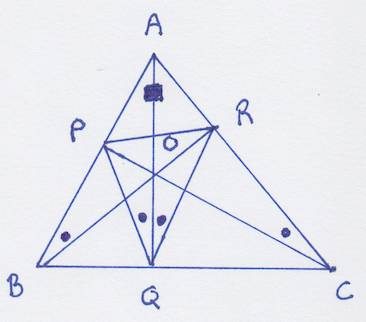
\includegraphics [scale=0.5] {T3.png} \end{center}
Here, we will show that when a triangle is drawn using the points where the altitudes hit the sides, those same lines bisect the angles of the new triangle.  Draw the altitudes in $\triangle ABC$ and join the points where the right angles are formed, along the bases, to give $\triangle PQR$.  The key is that the altitudes connect as right angles and they go through the orthocenter, which we have \emph{already shown to exist}.

Quadrilateral $ORCQ$ has two right angles at opposing vertices.  If we make $OC$ the diameter of a circle, then $R$ and $Q$ will have right angles.  This is a consequence of the inscribed angle theorem.
\begin{center} 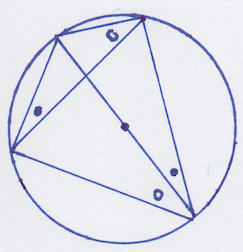
\includegraphics [scale=0.6] {T5.png} \end{center}
Here's an example.  The twisted kite (two short sides not equal, two long sides not equal either) is not symmetric.  Nevertheless, the angles marked with blue dots, as well as the pair marked with open circles, are equal.

So, in our original diagram, $\angle RCO$ and $\angle OQR$, are inscribed angles that subtend the same arc, so they are equal.  That accounts for two of the filled dots. 
\begin{center} 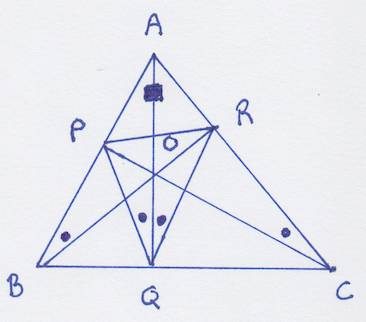
\includegraphics [scale=0.5] {T3.png} \end{center}
Either symmetry, or an equivalent circle construction for quadrilateral $OQBP$ will show that $\angle PBO$ and $\angle PQO$ sweep out the same arc, so they are equal as well.

But now consider $\triangle ABR$ and $\triangle APC$.  Both are right triangles that contain $\angle PAR$.  Therefore, the complementary angles in these two triangles are equal.  These are the two angles that are components of $\angle B$ and $\angle C$.  All four blue dotted angles are equal.

We conclude that $\angle PQR$ is bisected, which by symmetry, means that all the angles of $\triangle PQR$ are bisected.  

$O$ is both the incenter of the $\triangle PRQ$, the center of its incircle, and also the orthocenter of the original $\triangle ABC$.  Since the incenter certainly exists, this is yet another proof that the orthocenter exists.

We have proceeded first from circumcenter to orthocenter, and onward to incenter.

\subsection*{challenge}
This is our last problem in pure geometry.  See if you can prove it before reading further.
\begin{center} \includegraphics [scale=0.5] {bisectors_isosceles.png} \end{center}
Given that $\angle A$ and $\angle B$ are bisected.  If we also know that $\angle A = \angle B$ (isosceles $\triangle$), then it follows that the lengths of the bisectors are equal:  $AD = BE$.  This follows from ASA and $\triangle ABE \cong \triangle ADB$.

What about the converse?  Given $AD = BE$, show that the triangle is isosceles.  Draw the parallelogram $AEFD$.

\emph{Proof}.

By contradiction.  Suppose $\alpha > \beta$.  By the theorem of greater side $\iff$ greater angle, $AE > BD$.  But $AE = DF$ (parallelogram), so $DF > BD$.  By the converse theorem, $\phi > \theta$.
\begin{center} \includegraphics [scale=0.5] {bisectors_isosceles.png} \end{center}
Adding inequalities gives $\alpha + \phi > \beta + \theta$.  By the forward theorem, $EF > BE$.  Since $AD = EF$, $AD > BE$.  But this is a contradiction.

Assuming that $\beta > \alpha$ gives a similar contradiction by the symmetric construction.  Hence $\alpha = \beta$ and $2\alpha = 2\beta$.  $\square$

\end{document}
